\subsection{Topological manifolds}

\bd
A paracompact, Hausdorff, topological space $(M,\cO)$ is called a \emph{$d$-dimensional (topological) manifold}\index{manifold}\index{manifold!topological} if for every point $p\in M$ there exist a neighbourhood $U(p)$ and a homeomorphism $x\cl U(p) \to x(U(p)) \se \R^d$. We also write $\dim M = d$.
\ed

Intuitively, a $d$-dimensional\index{dimension!manifold} manifold is a topological space which locally (i.e.\ around each point) looks like $\R^d$.
\bp
Let $M$ be a $d$-dimensional manifold and let $U,V\se M$ be open, with $U\cap V \neq \vn$. If $x$ and $y$ are two homeomorphisms
\bse
x\cl U \to x(U)\se \R^d \qquad \text{and}\qquad y\cl V \to y(V)\se\R^{d'},
\ese
then $d=d'$.
\ep
This ensures that the concept of dimension is indeed well-defined, i.e.\ it is the same at every point, at least on each connected component of the manifold.

\be
Trivially, $\R^d$ is a $d$-dimensional manifold for any $d \geq 1$. The space $S^1$ is a 1-dimensional manifold while the spaces $S^2$, $C$ and $T^2$ are 2-dimensional manifolds.
\ee

\bd
Let $(M,\cO)$ be a topological manifold and let $N \se M$. Then $(N,\cO|_N)$ is called a \emph{submanifold} of $(M,\cO)$ if it is a manifold in its own right.
\ed

\be
The space $S^1$ is a submanifold of $\R^2$ while the spaces $S^2$, $C$ and $T^2$ are submanifolds of $\R^3$. 
\ee

\bd
Let $(M,\cO_M)$ and $(N,\cO_N)$ be topological manifolds of dimension $m$ and $n$, respectively. Then, $(M\times N,\cO_{M\times N})$ is a topological manifold of dimension $m+n$ called the \emph{product manifold}\index{manifold!product}.
\ed

\be
We have $T^2=S^1\times S^1$ not just as topological spaces, but as topological manifolds as well. This is a special case of the $n$-torus:
\bse
T^n := \underbrace{S^1\times S^1 \times \cdots \times S^1}_{\t{$n$ times}},
\ese
which is an $n$-dimensional manifold.
\ee

\be
The cylinder $C=S^1\times \R$ is a $2$-dimensional manifold.
\ee

\subsection{Bundles}

Products are very useful. Very often in physics one intuitively thinks of the product of two manifolds as attaching a copy of the second manifold to each point of the first.  However, not all interesting manifolds can be understood as products of manifolds. A classic example of this is the \emph{M\"obius strip}.


\bd
A \emph{bundle}\index{bundle} (of topological manifolds) is a triple $(E,\pi,M)$ where $E$ and $M$ are topological manifolds called the \emph{total space} and the \emph{base space} respectively, and $\pi$ is a continuous, surjective map $\pi\cl E \to M$ called the \emph{projection map}.
\ed

We will often denote the bundle $(E,\pi,M)$ by $E\xrightarrow{\,\pi\,}M$.

\bd
Let $E\xrightarrow{\,\pi\,}M$ be a bundle and let $p\in M$. Then, $F_p:=\mathrm{preim}_\pi(\{p\})$ is called the \emph{fibre}\index{fibre} at the point $p$.
\ed

Intuitively, the fibre at the point $p\in M$ is a set of points in $E$ (represented below as a line) attached to the point $p$. The projection map sends all the points is the fibre $F_p$ to the point $p$.

\begin{figure}[h!]
\centering
\begin{tikzpicture}[scale=0.8]
\draw  plot[smooth cycle, tension=.9] coordinates {(-3,1.5)(-1.5,2) (1,1.5) (3.5,-0.5) (5,-2) (2,-2) (0.5,-3)};
\node (v1) at (0,0) {};
\draw[dashed] plot[smooth, tension=.7] coordinates {(1,-1.5) (0,-1) (-0.5,-0.5) (v1)};
\draw  plot[smooth, tension=.7] coordinates {(v1) (0.5,0.5) (0.5,1) (0,2.5) (0,3.5)};
\draw[fill=black]  (v1) circle (0.08);
\node at (0.5,2.5) {$F_p$};
\node at (2.75,2) {$E$};
\node at (0.5,-0.5) {$p \in M$};
\node at (-2.5,1.5) {$M$};
\end{tikzpicture}
\end{figure}

\be
A trivial example of a bundle is the \emph{product bundle}. Let $M$ and $N$ be manifolds. Then, the triple $(M\times N,\pi,M)$, where:
\bi{rrCl}
\pi \cl & M\times N & \to & M\\
& (p,q) & \mapsto & p
\ei
is a bundle since (one can easily check) $\pi$ is a continuous and surjective map. Similarly, $(M\times N,\pi,N)$ with the appropriate $\pi$, is also a bundle.
\ee

\be
In a bundle, different points of the base manifold may have (topologically) different fibres. For example, consider the bundle $E\xrightarrow{\,\pi\,}\R$ where:
\bse
F_p:=\mathrm{preim}_\pi(\{p\}) \cong_\mathrm{top} \left\{ \ba{ll} S^1 &\t{if }p<0\\
\{p\} & \t{if }p=0\\ {}
[0,1] & \t{if } p>0 \ea \right.
\ese
\ee

\bd
Let $E\xrightarrow{\,\pi\,}M$ be a bundle and let $F$ be a manifold. Then, $E\xrightarrow{\,\pi\,}M$ is called a \emph{fibre bundle}\index{fibre bundle}\index{bundle!fibre}, with (typical) fibre $F$, if:
\bse
\forall \, p \in M : \mathrm{preim}_\pi(\{p\}) \cong_\mathrm{top} F.
\ese
\ed

A fibre bundle is often represented diagrammatically as:
\bse
\begin{tikzcd}
F\ar[r] & E \ar[d,"\pi"]\\
& M
\end{tikzcd}
\ese

\be
The bundle $M\times N\xrightarrow{\,\pi\,}M$ is a fibre bundle with fibre $F:=N$.
\ee

\be
The M\"obius strip is a fibre bundle $E\xrightarrow{\,\pi\,}S^1$, with fibre $F:=[0,1]$, where $E\neq S^1\times[0,1]$, i.e.\ the M\"obius strip is not a product bundle. 
\ee

\be
A $\C$-line bundle over $M$ is the fibre bundle $(E,\pi,M)$ with fibre $\C$. Note that the product bundle $(M\times \C,\pi,M)$ is a $\C$-line bundle over $M$, but a $\C$-line bundle over $M$ need not be a product bundle.
\ee

\bd
Let $E\xrightarrow{\,\pi\,}M$ be a bundle. A map $\s\cl M \to E$ is called a \emph{(cross-)section}\index{section} of the bundle if $\pi \circ \s = \id_M$.
\ed

Intuitively, a section is a map $\s$ which sends each point $p\in M$ to \emph{some} point $\s(p)$ in its fibre $F_p$, so that the projection map $\pi$ takes $\s(p) \in F_p\se E$ back to the point $p\in M$.


\begin{figure}[h!]
\centering
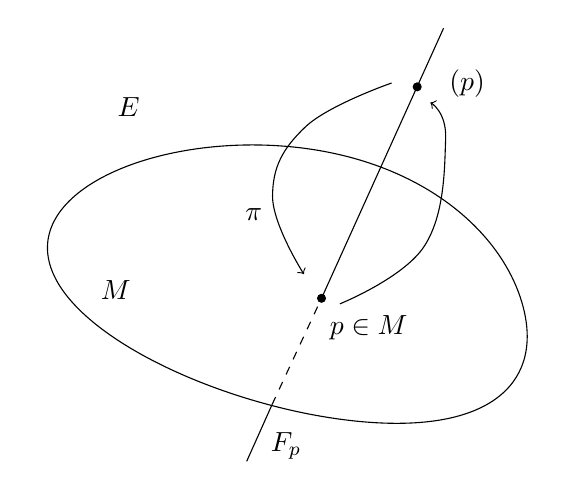
\begin{tikzpicture}[scale=1]
\draw  plot[smooth cycle, tension=.99] coordinates {(-2.5,0) (0.5,1.5) (3.5,-0.5) (1.5,-2)};
\draw (0,-2.5) -- (0.3224,-1.7792);
\draw[dashed]  (0.3224,-1.7792) -- (0.9501,-0.4298);
\draw (0.9501,-0.4298)-- (2.5,3);
\node at (0.5,-2.3) {$F_p$};
\node at (1.55,-0.8) {$p \in M$};
\draw[fill=black] (0.9501,-0.4298) circle (0.05);
\draw [->] plot[smooth, tension=.7] coordinates {(1.1834,-0.5006) (2.2576,0.2354) (2.5265,1.5914) (2.3316,2.0564)};
\draw [->] plot[smooth, tension=.7] coordinates {(1.8399,2.3042) (0.7458,1.7472) (0.3281,0.872) (0.7259,-0.1226)};
\node at (0.09,0.6333) {$\pi$};
\node at (1.8,0.2) {$\s$};
\node at (-1.6612,-0.3216) {$M$};
\draw [fill=black] (2.1651,2.2555) circle (0.05);
\node at (2.8,2.3) {$\s(p)$};
\node at (-1.5,2) {$E$};
\end{tikzpicture}
\end{figure}

\be
Let $(M\times F,\pi,M)$ be a product bundle. Then, a section of this bundle is a map:
\bi{rrCl}
\s \cl & M & \to & M\times F\\
& p & \mapsto & (p,s(p))
\ei
where $s\cl M \to F$ is any map.
\ee

\bd
A \emph{sub-bundle}\index{sub-bundle} of a bundle $(E,\pi,M)$ is a triple $(E',\pi',M')$ where $E'\se E$ and $M'\se M$ are submanifolds and $\pi':=\pi|_{E'}$.
\ed

\bd
Let $(E,\pi,M)$ be a bundle and let $N\se M$ be a submanifold. The \emph{restricted bundle}\index{bundle!restricted} (to $N$) is the triple $(E,\pi',N)$ where:
\bse
\pi':=\pi|_{\mathrm{preim}_\pi(N)}
\ese
\ed

\bd
Let $E\xrightarrow{\,\pi\,}M$ and $E'\xrightarrow{\,\pi'\,}M'$ be bundles and let $u\cl E\to E'$ and $v\cl M\to M'$ be maps. Then $(u,v)$ is called a \emph{bundle morphism}\index{morphism} if the following diagram commutes:
\bse
\begin{tikzcd}
E \ar[r,"u"] \ar[d,"\pi"]& E' \ar[d,"\pi'"]\\
M \ar[r,"v"]& M'
\end{tikzcd}
\ese
i.e.\ if $\pi'\circ u = v \circ \pi$.
\ed

If $(u,v)$ and $(u,v')$ are both bundle morphisms, then $v=v'$. That is, given $u$, if there exists $v$ such that $(u,v)$ is a bundle morphism, then $v$ is unique.

\bd
Two bundles $E\xrightarrow{\,\pi\,}M$ and $E'\xrightarrow{\,\pi'\,}M'$ are said to be \emph{isomorphic (as bundles)}\index{bundle!(locally) isomorphic} if there exist bundle morphisms $(u,v)$ and $(u^{-1},v^{-1})$ satisfying:
\bse
\begin{tikzcd}
E \ar[rr,shift left,"u"] \ar[dd,"\pi"']&& E' \ar[ll,shift left,"u^{-1}"]\ar[dd,"\pi'"]\\
&&\\
M \ar[rr,shift left,"v"]&& M' \ar[ll,shift left,"v^{-1}"]
\end{tikzcd}
\ese
Such a $(u,v)$ is called a \emph{bundle isomorphism}\index{isomorphism!of bundles}.
\ed

Bundle isomorphisms are the structure-preserving maps for bundles.

\bd
A bundle $E\xrightarrow{\,\pi\,}M$ is said to be \emph{locally isomorphic (as a bundle)} to a bundle $E'\xrightarrow{\,\pi'\,}M'$ if for all $p\in M$ there exists a neighbourhood $U(p)$ such that the restricted bundle:
\bse
\mathrm{preim}_\pi(U(p))\xrightarrow{\,\pi|_{\mathrm{preim}_\pi(U(p))}\,}U(p)
\ese
is isomorphic to the bundle $E'\xrightarrow{\,\pi'\,}M'$.
\ed

\bd
A bundle $E\xrightarrow{\,\pi\,}M$ is said to be:
\ben
\item[i)] \emph{trivial}\index{bundle!(locally) trivial} if it is isomorphic to a product bundle;
\item[ii)] \emph{locally trivial} if it is locally isomorphic to a product bundle.
\een
\ed

\be
The cylinder $C$ is trivial as a bundle, and hence also locally trivial.
\ee

\be
The M\"obious strip is not trivial but it is locally trivial.
\ee

From now on, we will mostly consider locally trivial bundles.

\br
In quantum mechanics, what is usually called a ``wave function'' is not a function at all, but rather a section of a $\C$-line bundle over physical space. However, if we assume that the $\C$-line bundle under consideration is locally trivial, then each section of the bundle can be represented (locally) by a map from the base space to the total space and hence it is appropriate to use the term ``wave \emph{function}''. 
\er

\bd
Let $E\xrightarrow{\,\pi\, }M$ be a bundle and let $f\cl M'\to M$ be a map from some manifold $M'$. The \emph{pull-back bundle of} \index{bundle!pull-back}$E\xrightarrow{\,\pi\, }M$ \emph{induced by} $f$ is defined as $E'\xrightarrow{\,\pi'\,}M'$, where:
\bse
E':=\{(m',e)\in M'\times E \mid f(m')=\pi(e)\}
\ese
and $\pi' (m',e) := m'$.
\ed

If $E'\xrightarrow{\,\pi'\,}M'$ is the pull-back bundle of $E\xrightarrow{\,\pi\, }M$ induced by $f$, then one can easily construct a bundle morphism by defining:
\bi{rcCl}
u \cl & E'  & \to & E\\
& (m',e) & \mapsto & e
\ei
This corresponds to the diagram:
\bse
\begin{tikzcd}
E' \ar[d,"\pi'"] \ar[r,"u"] & E\ar[d,"\pi"]\\
M' \ar[r,"f"]& M
\end{tikzcd}
\ese

\br
Sections on a bundle pull back to the pull-back bundle. Indeed, let $E'\xrightarrow{\,\pi'\,}M'$ be the pull-back bundle of $E\xrightarrow{\,\pi\, }M$ induced by $f$.
\bse
\begin{tikzcd}
E' \ar[dd,shift left,"\pi'"] && E\ar[dd,shift left,"\pi"]\\
&&\\
M' \ar[uurr,"\s\circ f"]\ar[uu,shift left,"\s'"]\ar[rr,"f"]&& M\ar[uu,shift left,"\s"]
\end{tikzcd}
\ese
If $\s$ is a section of $E\xrightarrow{\,\pi\, }M$, then $\s \circ f$ determines a map from $M'$ to $E$ which sends each $m'\in M'$ to $\s(f(m')) \in E$. However, since $\s$ is a section, we have:
\bse
\pi(\s(f(m'))= (\pi \circ \s \circ f)(m') = (\id_M\circ f)(m') = f(m')
\ese
and hence $(m',(\s \circ f)(m'))\in E'$ by definition of $E'$. Moreover:
\bse
\pi' (m',(\s \circ f)(m')) = m'
\ese
and hence the map:
\bi{rcCl}
\s' \cl & M'  & \to & E'\\
& m' & \mapsto & (m',(\s \circ f)(m'))
\ei
satisfies $\pi'\circ\s'=\id_{M'}$ and it is thus a section on the pull-back bundle $E'\xrightarrow{\,\pi'\,}M'$.
\er

\subsection{Viewing manifolds from atlases}

\bd
Let $(M,\cO)$ be a $d$-dimensional manifold. Then, a pair $(U,x)$ where $U\in \cO$ and $x\cl U \to x(U) \se \R^d$ is a homeomorphism, is said to be a \emph{chart}\index{chart} of the manifold.
\ed

The \emph{component functions (or maps)}\index{component map}\index{map!component} of $x\cl U\to x(U) \se \R^d$ are the maps:
\bi{rcCl}
x^i \cl & U  & \to & \R\\
& p & \mapsto & \proj_i(x(p))
\ei
for $1\leq i\leq d$, where $\mathrm{proj}_i(x(p))$ is the $i$-th component of $x(p)\in \R^d$. The $x^i(p)$ are called the \emph{co-ordinates}\index{co-ordinates} of the point $p\in U$ with respect to the chart $(U,x)$.

\bd
An \emph{atlas}\index{atlas} of a manifold $M$ is a collection $\mathscr{A}:=\{(U_\a,x_\a)\mid \a \in \mathcal{A}\}$ of charts such that:
\bse
\bigcup_{\a \in \mathcal{A}}U_\a = M. 
\ese
\ed

\bd
Two charts $(U,x)$ and $(V,y)$ are said to be \emph{$C^0$-compatible} if either $U \cap V = \vn$ or the map:
\bse
y\circ x^{-1}\cl x(U\cap V) \to y(U\cap V)
\ese
is continuous.
\ed

Note that $y\circ x^{-1}$ is a map from a subset of $\R^d$ to a subset of $\R^d$.
\bse
\begin{tikzcd}
& U\cap V \se M \ar[ldd,"x"'] \ar[rdd,"y"]&\\
&&&\\
x(U\cap V) \se \R^d \ar[rr,"y\circ x^{-1}"']& & y(U\cap V)\se \R^d
\end{tikzcd}
\ese

Since the maps $x$ and $y$ are homeomorphisms, the composition map $y \circ x^{-1}$ is also a homeomorphism and hence continuous. Therefore, any two charts on a topological manifold are $C^0$-compatible. This definition my thus seem redundant since it applies to every pair of charts. However, it is just a ``warm up'' since we will later refine this definition and define the \emph{differentiability} of maps on a manifold in terms of $C^k$-compatibility of charts. 

\br
The map $y\circ x^{-1}$ (and its inverse $x\circ y^{-1}$) is called the \emph{co-ordinate change map} or \emph{chart transition map}\index{map!transition}.
\er

\bd
A \emph{$C^0$-atlas} of a manifold is an atlas of pairwise $C^0$-compatible charts.
\ed

Note that any atlas is also a \emph{$C^0$-atlas}.

\bd
A $C^0$-atlas $\mathscr{A}$ is said to be a \emph{maximal atlas} if for every $(U,x)\in\mathscr{A}$, we have $(V,y)\in\mathscr{A}$ for all $(V,y)$ charts that are $C^0$-compatible with $(U,x)$.
\ed

\be
Not every $C^0$-atlas is a maximal atlas. Indeed, consider $(\R,\cO_\mathrm{std})$ and the atlas $\mathscr{A}:=(\R,\id_\R)$. Then $\mathscr{A}$ is not maximal since $((0,1),\id_\R)$ is a chart which is $C^0$-compatible with $(\R,\id_\R)$ but $((0,1),\id_\R) \notin \mathscr{A}$.
\ee

We can now look at ``objects on'' topological manifolds from two points of view. For instance, consider a curve on a $d$-dimensional manifold $M$, i.e.\ a map $\g\cl \R\to M$. We now ask whether this curve is continuous, as it should be if models the trajectory of a particle on the ``physical space'' $M$.

A first answer is that $\g\cl \R \to M$ is continuous if it is continuous as a map between the topological spaces $\R$ and $M$.

However, the answer that may be more familiar to you from undergraduate physics is the following. We consider only a portion (open subset $U$) of the physical space $M$ and, instead of studying the map $\g\cl\mathrm{preim}_\g(U)\to U$ directly, we study the map:
\bse
x\circ \g\cl \mathrm{preim}_\g(U) \to x(U) \se \R^d,
\ese
where $(U,x)$ is a chart of $M$. More likely, you would be checking the continuity of the co-ordinate maps $x^i\circ \g$, which would then imply the continuity of the ``real'' curve $\g\cl\mathrm{preim}_\g(U)\to U$ (real, as opposed to its co-ordinate representation).
\bse
\begin{tikzcd}
&& y(U)\se\R^d\\
&&\\
\mathrm{preim}_\g(U)\se\R \ar[rr,"\g"] \ar[ddrr,"x\circ \g"] \ar[uurr,"y\circ \g"]&& U\se M \ar[dd,"x"] \ar[uu,"y"'] \\
&&\\
&& x(U)\se\R^d \ar[uuuu,bend right=65,"y\circ x^{-1}"']
\end{tikzcd}
\ese
At some point you may wish to use a different ``co-ordinate system'' to answer a different question. In this case, you would chose a different chart $(U,y)$ and then study the map $y\circ \g$ or its co-ordinate maps. Notice however that some results (e.g.\ the continuity of $\g$) obtained in the previous chart $(U,x)$ can be immediately ``transported'' to the new chart $(U,y)$ via the chart transition map $y\circ x^{-1}$. Moreover, the map $y\circ x^{-1}$ allows us to, intuitively speaking, forget about the inner structure (i.e.\ $U$ and the maps $\g$, $x$ and $x$) which, in a sense, is the real world, and only consider $\mathrm{preim}_\g(U)\se \R$ and $x(U),y(U)\se\R^d$ together with the maps between them, which is our representation of the real world.














